%%%%%%%%%%%%%%%%%%%%%%%%%%%%%%%%%%%%%%%%%
% Research Report Assignment Title Page 
% LaTeX Template
% Version 1.0 (06/03/16)
%
% This template has been downloaded from:
% http://www.LaTeXTemplates.com
%
% Original author: Francisco Maria Calisto
% WikiBooks (http://en.wikibooks.org/wiki/LaTeX/Title_Creation)
%
% License:
% CC BY-NC-SA 3.0 (http://creativecommons.org/licenses/by-nc-sa/3.0/)
% 
% Instructions for using this template:
% This title page is capable of being compiled as is. This is not useful for 
% including it in another document. To do this, you have two options: 
%
% 1) Copy/paste everything between \begin{document} and \end{document} 
% starting at \begin{titlepage} and paste this into another LaTeX file where you 
% want your title page.
% OR
% 2) Remove everything outside the \begin{titlepage} and \end{titlepage} and 
% move this file to the same directory as the LaTeX file you wish to add it to. 
% Then add \input{./title_page_1.tex} to your LaTeX file where you want your
% title page.
%
%%%%%%%%%%%%%%%%%%%%%%%%%%%%%%%%%%%%%%%%%
%\title{Title page with logo}
%------------------------------------------------------------------------------
%	PACKAGES AND OTHER DOCUMENT CONFIGURATIONS
%------------------------------------------------------------------------------

\documentclass[12pt]{article}
\usepackage[english]{babel}
\usepackage[utf8x]{inputenc}
\usepackage[T1]{fontenc}
\usepackage{amsmath}
\usepackage{graphicx}
\usepackage[colorinlistoftodos]{todonotes}
\usepackage{subcaption}
\usepackage{biblatex}
\usepackage{fontspec}
\usepackage{pifont}

\addbibresource{bib.bib}

\begin{document}

\begin{titlepage}

\newcommand{\HRule}{\rule{\linewidth}{0.5mm}} % Defines a new command for the horizontal lines, change thickness here

\center % Center everything on the page
 
%------------------------------------------------------------------------------
%	HEADING SECTIONS
%------------------------------------------------------------------------------

% Name of your university/college
\textsc{\LARGE Instituto Superior T\'{e}cnico}\\[1.5cm]
% Major heading such as course name
\textsc{\Large ISR}\\[0.5cm]
% First Minor heading such as course title
\textsc{\large Report}\\[0.25cm]
% Second Minor heading such as course title
\textsc{\small Users and Tasks Analysis Milestone}\\[0.25cm]

%------------------------------------------------------------------------------
%	TITLE SECTION
%------------------------------------------------------------------------------

\HRule \\[0.5cm]
{ \large \bfseries Participatory User Tests Meeting \& Notes}\\[0.25cm] % Title of your document
\HRule \\[0.5cm]
 
%------------------------------------------------------------------------------
%	AUTHOR SECTION
%------------------------------------------------------------------------------

\begin{minipage}{0.4\textwidth}
\begin{flushleft} \large
\emph{Author:}\\
Francisco Maria \textsc{Calisto} % Your name
\end{flushleft}
\end{minipage}
~
\begin{minipage}{0.4\textwidth}
\begin{flushright} \large
\emph{Coordinator:} \\
Jacinto \textsc{Nascimento} % Coordinator's Name
\end{flushright}
~
\begin{flushright} \large
\emph{Co-Coordinator:} \\
Daniel \textsc{Gon\c{c}alves} % Co-Coordinator's Name
\end{flushright}
\end{minipage}\\[2cm]

% If you don't want a supervisor, uncomment the two lines below and remove the section above
%\Large \emph{Author:}\\
%John \textsc{Smith}\\[3cm] % Your name

%-----------------------------------------------------------------------------
%	DATE SECTION
%-----------------------------------------------------------------------------

{\large 20/02/2017}\\[1cm] % Date, change the \today to a set date if you want to be precise

%-----------------------------------------------------------------------------
%	LOGO SECTION
%-----------------------------------------------------------------------------

% 
\includegraphics{ist-logo.png}\\[0.5cm] % Include a department/university logo - this will require the graphicx package

% 
\includegraphics{isr-logo.png}\\[0.5cm] % Include a department/university logo - this will require the graphicx package

\begin{figure}
\centering
\begin{subfigure}{.5\textwidth}
  \centering
  
\includegraphics[width=.5\linewidth]{isr-logo.png}
\end{subfigure}%
\begin{subfigure}{.5\textwidth}
  \centering
  
\includegraphics[width=.5\linewidth]{inesc-id-logo.png}
\end{subfigure}
\begin{subfigure}{.5\textwidth}
  \centering
  
\includegraphics[width=.25\linewidth]{ist-logo.png}
\end{subfigure}
\end{figure}
 
%-----------------------------------------------------------------------------

\vfill % Fill the rest of the page with whitespace

\end{titlepage}

\section{Abstract}

This report will prepare us to better understand what is the best approach as an user and task analysis in a clinical environment. This way we will have a vision of how we should test our interface and how to get the best feedback from clinicians.

\section{Introduction}

As a researcher, we have been told countless times that user feedback is an important key to understand the user goals and tasks to achieve. The benefits of testing a product with users are obviously positive and conclusive. While this kind of information provide good advice on how the test is done, they often lack explanations on how a testing process fits inside a team and how to make sense of this feedback.

For this phase we have prepared a script test that will help us understanding the tasks and will be our guide so that the test is always unanimous even if we take a more open and not strict approach to the script.

\clearpage

\section{Interactive Design}

- How many users we need?

When working on the research and development of a new user interface, we need to iterate with several test sessions to check our development choices. Each of this sessions consist in testing the user with 3 individual clinic testers (until this date). What we have experienced is that we do not actually need a huge set of people, like 10 testers, to identify an issue. With 3 tests, we can already see what are recurring problems with almost a 75\% of usability problems found, which corroborates Nielsen’s graph \cite{needTest} (Figure 2).

% Commands to include a figure:
\begin{figure}[!hbt]
\centering
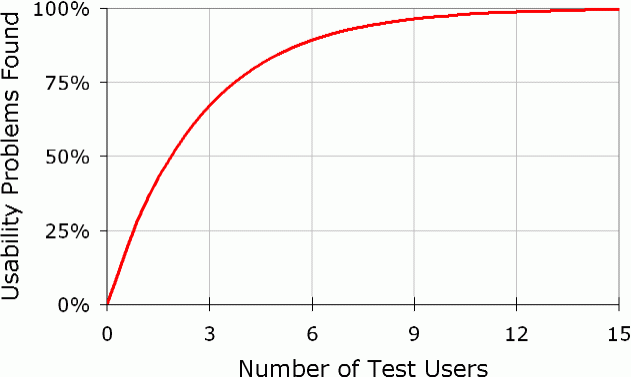
\includegraphics[width=1.0\textwidth]{number-of-test-users.png}
\caption{\label{fig:frog}User Tests}
\end{figure}

We usually met the users on their office since they have the material diagnostic with them and to observe the behaviour on their environment. We give them our machines to show the prototypes or just have an open interview to make some questions about the goals and the tasks to be concluded. It is important that each time we prepare a new user test session, we meet to define the learning goals, i.e. assumptions that need to be verified or might be proven wrong. For instance, when observing the clinic on their behaviour we understood the less usage of the keyboard against a very used mouse features.

\clearpage

\section{Learning Goals}

The learning goals are:

- Understand how to annotate breast mass on our prototype;

- Understand how to annotate breast calcification on our prototype;

- Understand how to undo some annotation;

- Understand how to redo some action on the prototype;

- Understand how to erase some annotation on the prototype;

\section{Phase Validation}

- What needs to be validate on this phase?

\section{Interviews vs Surveys}

- Does it make sense to mix from Interviews and Surveys?

\section{Script}

Before the users test, the research writes a script that will serve as a roadmap and guideline that can be shared with all research team who lead this project. It is a way to have consistent and comparable results.

This script consists in:

\ding{226} A reminder of the learning goals.

\ding{226} A check-list of the set-up elements that should be available for the test.

\ding{226} A clear and objective task: the job the clinician has to complete. It generally implies achieving smaller tasks related to the learning goals.

\ding{226} A few demographic questions to ask at the end.

On this research phase we will strict the interaction with the user as a beginning phase to record and obtain a new preliminary information about the user needs, goals and tasks. However we already tested some prototypes with Dra. Cristina Ribeiro da Fonseca and Dra. Clara Aleluia, it is still possible and valuable to restart the all process.

\clearpage

\section{Paper}

\subsection{Motivation}

\subsection{Solving A Problem}

\subsection{The Paper Solution}

\subsection{Where To Publish The Paper?}

\subsection{Clinical Conferences and Journals Research}

\section{Tasks}

- Find the ways how to detect false positives.

\section{Questions}

The following questions were made to the clinicians:

- Ask the question about having the BIRAD in each diagnosis image?

- Is it better on the High-Fi Prototype to have the right-click with all option, just the right menu with the options or both?

- Is it useful to have the colours annotation option?

\clearpage

\section{Conclusions}

\clearpage

\section{Acknowledgements}

This report will help our research project in cooperation between ISR \cite{isr} and INESC-ID \cite{inescid} both are associate institutes of Instituto Superior T\'{e}cnico \cite{ist}, Universidade de Lisboa \cite{ul}. Throughout this challenging journey we had the untiring and patient support from our family and friends.

We would like to give a special thanks to Dr. Cristina Ribeiro da Fonseca and Dr. Clara Aleluia who have cooperated with us tirelessly, thus making a major contribution to the national research and development of innovation in Portuguese clinical Information Systems.

We also want to thanks Bruno Cardoso, Rodrigo Louren\c{c}o, Bruno Oliveira, Tom\'{a}s Pinho, L\'{i}dia Freitas, Bruno Dias, Jo\~{a}o Miranda, Prof. Dr. Jacinto Nascimento, Prof. Dr. Daniel Gon\c{c}alves, Ana Beatriz Alves, Francisco Silveira, Joana Teixeira, Daniel Da Costa, Filipe Fernandes, In\^{e}s Fran\c{c}a Martins, Lu\'{i}s Ribeiro Gomes and Ricardo Cruz for helping, supporting and reviewing our work.

\clearpage

\printbibliography

\end{document}
